\documentclass[10pt,journal,compsoc,onecolumn]{IEEEtran}
\usepackage[utf8]{inputenc}
\usepackage{amsmath,amsfonts,amssymb}
\usepackage{amsthm}
\usepackage{graphicx}
\usepackage{cite}
\usepackage{textcomp}
\usepackage{tikz}
\usetikzlibrary{arrows,positioning,shapes.geometric}
\usepackage{booktabs}
\usepackage{url}

\newtheorem{theorem}{Theorem}
\newtheorem{lemma}[theorem]{Lemma}
\newtheorem{definition}[theorem]{Definition}
\newtheorem{corollary}[theorem]{Corollary}

\begin{document}

\title{A Formal Algorithmic Analysis of Queue Data Structures: Implementations, Deques, and Sliding Window Maximum Optimizations}

\IEEEtitleabstractindextext{%
\begin{abstract}
Queues represent a fundamental linear data structure operating under the First-In, First-Out (FIFO) protocol. This paper presents a formal analysis and reference implementations of queue structures using dynamic arrays and singly-linked lists, detailing their performance bounds. We investigate circular buffer representations using modular arithmetic to achieve constant-time operations. We also formalize the implementation of a queue using two stacks, establishing their amortized complexity bounds. Finally, we explore the Sliding Window Maximum problem, demonstrating how the Monotonic Deque paradigm reduces the naive $O(N \cdot K)$ brute-force solution to an optimal $O(N)$ time complexity. Complete implementations in Java and formal correctness arguments are provided.
\end{abstract}

\begin{IEEEkeywords}
linked list, deep copy, random pointer, hash map, node interleaving, Java, algorithm analysis, computational complexity
\end{IEEEkeywords}
}

\maketitle
\IEEEdisplaynontitleabstractindextext
\IEEEpeerreviewmaketitle

\section{Introduction}
Linear data structures form the foundation of computer science, providing structured mechanisms for memory management and element access. While the Stack data structure operates under the Last-In, First-Out (LIFO) access pattern, the Queue data structure enforces a First-In, First-Out (FIFO) order. In a FIFO structure, the element that has been in the queue for the longest duration is the first to be removed.

Queues are utilized in a variety of systems programming and network design scenarios:
\begin{itemize}
    \item \textbf{Operating System Scheduling:} Ready queues manage processes awaiting CPU execution (e.g., Round-Robin scheduling).
    \item \textbf{Network Packet Buffering:} Routers maintain packets in transmission queues to regulate bandwidth allocation.
    \item \textbf{Asynchronous Task Management:} Message brokers (e.g., RabbitMQ, Kafka) utilize message queues to decouple distributed services.
    \item \textbf{Algorithm Design:} Breadth-First Search (BFS) uses a queue to traverse graphs layer by layer.
\end{itemize}

This paper provides a rigorous algorithmic treatment of queues. Section~\ref{sec:queue_adt} details the Queue Abstract Data Type (ADT) and its mathematical states. Section~\ref{sec:array_queue} and Section~\ref{sec:linked_list_queue} analyze array-based (circular) and linked-list-based queue implementations. Section~\ref{sec:stack_queue} formalizes a queue implementation using two stacks with an amortized complexity proof. Section~\ref{sec:deque} discusses the Doubly Ended Queue (Deque). Finally, Section~\ref{sec:sliding_window} details the Sliding Window Maximum problem, presenting an optimal $O(N)$ solver using a Monotonic Deque.

\section{Queue Abstract Data Type (ADT)}
\label{sec:queue_adt}
A queue $Q$ is a sequence of elements supporting restricted boundaries. Let $Q = \langle q_1, q_2, \ldots, q_n \rangle$ represent the queue, where $q_1$ is at the front (head) and $q_n$ is at the rear (tail).

The Queue ADT supports the following primary operators:
\begin{itemize}
    \item $\mathrm{Enqueue}(Q, x)$: Inserts element $x$ at the rear.
    $\langle q_1, \ldots, q_n \rangle \xrightarrow{\mathrm{enqueue}(x)} \langle q_1, \ldots, q_n, x \rangle$.
    \item $\mathrm{Dequeue}(Q)$: Removes and returns the front element $q_1$.
    $\langle q_1, \ldots, q_n \rangle \xrightarrow{\mathrm{dequeue}()} \langle q_2, \ldots, q_n \rangle$.
    \item $\mathrm{Peek}(Q)$: Returns the front element $q_1$ without altering the queue.
    \item $\mathrm{IsEmpty}(Q)$: Returns true if $n = 0$, else false.
\end{itemize}

\begin{figure}[htbp]
\centering
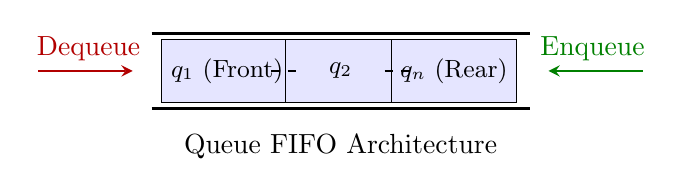
\begin{tikzpicture}[
  queuenode/.style={draw, rectangle, minimum width=1.4cm, minimum height=0.8cm, fill=blue!10, font=\small},
  scale=0.8
]
% Draw horizontal queue boundaries
\draw[very thick] (0, 0) -- (6.0, 0);
\draw[very thick] (0, 1.2) -- (6.0, 1.2);

% Draw elements
\node[queuenode] at (1.2, 0.6) {$q_1$ (Front)};
\node[queuenode] at (3.0, 0.6) {$q_2$};
\node[queuenode] at (4.8, 0.6) {$q_n$ (Rear)};

% Enqueue / Dequeue arrows
\draw[<-, >=stealth, thick, red!70!black] (-0.3, 0.6) -- (-1.8, 0.6);
\node[above, red!70!black] at (-1.0, 0.6) {Dequeue};

\draw[<-, >=stealth, thick, green!50!black] (6.3, 0.6) -- (7.8, 0.6);
\node[above, green!50!black] at (7.0, 0.6) {Enqueue};

\draw[dashed] (1.9, 0.6) -- (2.3, 0.6);
\draw[dashed] (3.7, 0.6) -- (4.1, 0.6);

\node at (3.0, -0.6) {Queue FIFO Architecture};
\end{tikzpicture}
\caption{Visual representation of a Queue operating under the First-In, First-Out (FIFO) principle.}
\label{fig:queue_adt}
\end{figure}

Table~\ref{tab:queue_complexities} summarizes the asymptotic time and space bounds for different queue designs.

\begin{table}[htbp]
\centering
\caption{Asymptotic Complexity of Queue Implementations.}
\label{tab:queue_complexities}
\begin{tabular}{lccc}
\toprule
Operation & Array-based (Shifting) & Circular Array & Linked List-based \\
\midrule
Enqueue & $O(1)$ amortized & $O(1)$ worst-case & $O(1)$ worst-case \\
Dequeue & $O(N)$ worst-case & $O(1)$ worst-case & $O(1)$ worst-case \\
Peek & $O(1)$ worst-case & $O(1)$ worst-case & $O(1)$ worst-case \\
Space Complexity & $O(N)$ total & $O(N)$ total & $O(N)$ total \\
Auxiliary Space & $O(1)$ & $O(1)$ & $O(1)$ \\
\bottomrule
\end{tabular}
\end{table}

\section{Array-Based Queue Implementation}
\label{sec:array_queue}
Implementing a queue using a static array of size $C$ requires careful indexing. If dequeue always returns the element at index $0$, then all remaining elements must shift left by one spot, incurring an $O(N)$ cost.

To achieve $O(1)$ time complexity for both enqueue and dequeue operations, we utilize a \emph{Circular Queue} model. We maintain a front cursor $f$ and a rear cursor $r$, initialized such that the queue is empty. By treating the array as a closed loop and using modular arithmetic, pointers advance circularly:
\begin{align}
    \mathrm{rear} &\leftarrow (\mathrm{rear} + 1) \bmod C \\
    \mathrm{front} &\leftarrow (\mathrm{front} + 1) \bmod C
\end{align}

\subsection{Java Implementation}
The Java implementation of a circular array queue is as follows:
\begin{verbatim}
public class CircularQueue {
    private final int[] arr;
    private int front;
    private int rear;
    private int size;
    private final int capacity;

    public CircularQueue(int capacity) {
        this.capacity = capacity;
        this.arr = new int[capacity];
        this.front = 0;
        this.rear = -1;
        this.size = 0;
    }

    public boolean enqueue(int x) {
        if (isFull()) {
            return false; // Queue Overflow
        }
        rear = (rear + 1) % capacity;
        arr[rear] = x;
        size++;
        return true;
    }

    public int dequeue() {
        if (isEmpty()) {
            return -1; // Queue Underflow
        }
        int val = arr[front];
        front = (front + 1) % capacity;
        size--;
        return val;
    }

    public int peek() {
        if (isEmpty()) {
            return -1;
        }
        return arr[front];
    }

    public boolean isEmpty() {
        return size == 0;
    }

    public boolean isFull() {
        return size == capacity;
    }
}
\end{verbatim}

\section{Singly-Linked List Queue Implementation}
\label{sec:linked_list_queue}
A linked list queue avoids the fixed-capacity limitations of arrays. We maintain reference pointers to the start and end of the list:
\begin{itemize}
    \item \textbf{head pointer:} Points to the front node. Dequeue operations occur here.
    \item \textbf{tail pointer:} Points to the rear node. Enqueue operations occur here.
\end{itemize}

\subsection{Java Implementation}
The Java implementation of a linked list queue is as follows:
\begin{verbatim}
public class LinkedListQueue {
    private static class Node {
        int data;
        Node next;
        Node(int data) {
            this.data = data;
            this.next = null;
        }
    }

    private Node head;
    private Node tail;

    public LinkedListQueue() {
        this.head = null;
        this.tail = null;
    }

    public void enqueue(int x) {
        Node newNode = new Node(x);
        if (tail == null) {
            head = newNode;
            tail = newNode;
            return;
        }
        tail.next = newNode;
        tail = newNode;
    }

    public int dequeue() {
        if (head == null) {
            return -1; // Underflow
        }
        int data = head.data;
        head = head.next;
        if (head == null) {
            tail = null; // List became empty
        }
        return data;
    }

    public int peek() {
        if (head == null) {
            return -1;
        }
        return head.data;
    }

    public boolean isEmpty() {
        return head == null;
    }
}
\end{verbatim}

\section{Queue Realization Using Stacks}
\label{sec:stack_queue}
A common algorithmic problem is implementing a queue using two stacks, \texttt{st1} and \texttt{st2}. This design achieves a FIFO interface using LIFO containers.

\subsection{Algorithm Description}
We designate \texttt{st1} as the primary enqueue target and \texttt{st2} as the dequeue source:
\begin{itemize}
    \item \textbf{Enqueue(x):} Push $x$ onto \texttt{st1}.
    \item \textbf{Dequeue():}
        \begin{enumerate}
            \item If both \texttt{st1} and \texttt{st2} are empty, throw an underflow exception.
            \item If \texttt{st2} is empty, transfer all elements from \texttt{st1} to \texttt{st2} by popping from \texttt{st1} and pushing to \texttt{st2}. This reverses the elements' order, transforming LIFO order to FIFO.
            \item Pop and return the top element of \texttt{st2}.
        \end{enumerate}
\end{itemize}

\subsection{Java Implementation}
The Java implementation of the stack-based queue is as follows:
\begin{verbatim}
import java.util.Stack;

public class StackQueue {
    private final Stack<Integer> st1 = new Stack<>();
    private final Stack<Integer> st2 = new Stack<>();

    public void enqueue(int x) {
        st1.push(x);
    }

    public int dequeue() {
        if (isEmpty()) {
            return -1; // Underflow
        }
        if (st2.isEmpty()) {
            while (!st1.isEmpty()) {
                st2.push(st1.pop());
            }
        }
        return st2.pop();
    }

    public int peek() {
        if (isEmpty()) {
            return -1;
        }
        if (st2.isEmpty()) {
            while (!st1.isEmpty()) {
                st2.push(st1.pop());
            }
        }
        return st2.peek();
    }

    public boolean isEmpty() {
        return st1.isEmpty() && st2.isEmpty();
    }
}
\end{verbatim}

\subsection{Complexity Analysis and Amortized Proof}
\begin{theorem}
In a two-stack queue implementation, the amortized time complexity of the Dequeue operation is $O(1)$.
\end{theorem}
\begin{proof}
Let $N$ be the number of elements processed by the queue. We analyze the total operations performed on the underlying stacks:
\begin{enumerate}
    \item Each element is pushed onto \texttt{st1} exactly once during Enqueue.
    \item Each element is popped from \texttt{st1} exactly once during the transfer step.
    \item Each element is pushed onto \texttt{st2} exactly once during the transfer step.
    \item Each element is popped from \texttt{st2} exactly once during Dequeue.
\end{enumerate}
Across the complete lifecycle of $N$ elements, the total stack push and pop operations are bounded by $4N$. Since each individual stack push or pop takes $O(1)$ time, the cumulative time for all operations is $O(N)$. Distributing this cost over $N$ dequeue operations yields an amortized time complexity of $O(1)$ per operation.
\end{proof}

\section{Doubly Ended Queue (Deque)}
\label{sec:deque}
A Doubly Ended Queue (Deque) is a generalization of a queue that supports insertion and deletion at both the front and the rear. 

The primary operations of a Deque are:
\begin{itemize}
    \item \texttt{insertFirst(x)}: Inserts element $x$ at the front.
    \item \texttt{insertLast(x)}: Inserts element $x$ at the rear (equivalent to Enqueue).
    \item \texttt{removeFirst()}: Removes and returns the front element (equivalent to Dequeue).
    \item \texttt{removeLast()}: Removes and returns the rear element.
\end{itemize}

A Deque can be implemented in $O(1)$ time for all operations using either a Circular Array with two active cursors or a Doubly Linked List, where each node has pointers to its predecessor and successor.

\section{Sliding Window Maximum and Monotonic Deques}
\label{sec:sliding_window}
The Sliding Window Maximum problem is a classic application of Deques.

\subsection{Problem Statement}
Given an integer array $A$ of size $N$ and a sliding window of size $K$ ($1 \le K \le N$), we find the maximum value in each contiguous subarray of size $K$. There are exactly $N - K + 1$ such windows.

\subsection{Brute-Force vs. Optimized Monotonic Solver}
A brute-force solution checks every window and searches for its maximum element:
\begin{verbatim}
// Brute Force: O(N * K)
public int[] bruteForce(int[] A, int K) {
    int[] res = new int[A.length - K + 1];
    for (int i = 0; i <= A.length - K; i++) {
        int max = A[i];
        for (int j = i; j < i + K; j++) {
            max = Math.max(max, A[j]);
        }
        res[i] = max;
    }
    return res;
}
\end{verbatim}
In the worst case (e.g., $K \approx N/2$), the time complexity is quadratic: $O(N \cdot K) \approx O(N^2)$.

To achieve an optimal linear time complexity, we maintain a Deque of array indices. The indices are stored such that their corresponding array values are in strictly decreasing order.
When processing element $A[i]$:
\begin{enumerate}
    \item We pop indices from the front of the Deque if they are out of the current window (i.e., index $< i - K + 1$).
    \item We pop indices from the rear of the Deque if their values are less than or equal to $A[i]$ (i.e., $A[\mathrm{idx}] \le A[i]$), as these elements are redundant for the current and any future window.
    \item We append the current index $i$ to the rear of the Deque.
    \item The maximum value of the active window is always located at the front of the Deque.
\end{enumerate}

\subsection{Illustrative Execution Trace}
We trace the evaluation of $A = [3, 2, 3, 4, 5, 5, 4, 5, 6]$ with window size $K = 4$ in Table~\ref{tab:trace_sliding}.

\begin{table}[htbp]
\centering
\caption{Dry-run trace of Sliding Window Maximum algorithm for $K=4$.}
\label{tab:trace_sliding}
\begin{tabular}{cllll}
\toprule
Step $i$ & $A[i]$ & Deque State (indices / values) & Output Max & Action Comments \\
\midrule
0 & 3 & $\langle 0 / (3) \rangle$ & -- & Push index 0 \\
1 & 2 & $\langle 0/(3), 1/(2) \rangle$ & -- & Push index 1 \\
2 & 3 & $\langle 2 / (3) \rangle$ & -- & Pop index 1 (val 2 $\le$ 3), pop index 0 (val 3 $\le$ 3) \\
3 & 4 & $\langle 3 / (4) \rangle$ & $A[3] = 4$ & Pop index 2 (val 3 $\le$ 4), push index 3 \\
4 & 5 & $\langle 4 / (5) \rangle$ & $A[4] = 5$ & Pop index 3 (val 4 $\le$ 5), push index 4 \\
5 & 5 & $\langle 5 / (5) \rangle$ & $A[5] = 5$ & Pop index 4 (val 5 $\le$ 5), push index 5 \\
6 & 4 & $\langle 5/(5), 6/(4) \rangle$ & $A[5] = 5$ & Push index 6 (val 4 $<$ 5) \\
7 & 5 & $\langle 7 / (5) \rangle$ & $A[7] = 5$ & Pop index 6, pop index 5, push index 7 \\
8 & 6 & $\langle 8 / (6) \rangle$ & $A[8] = 6$ & Pop index 7, push index 8 \\
\bottomrule
\end{tabular}
\end{table}

\begin{figure}[htbp]
\centering
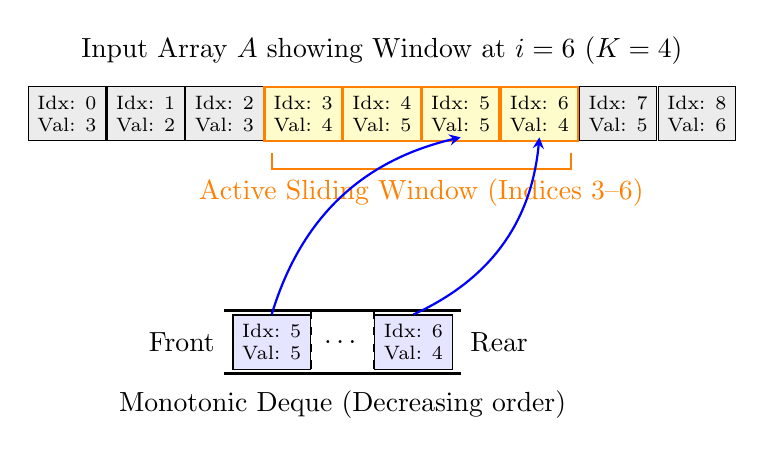
\begin{tikzpicture}[
  box/.style={draw, rectangle, minimum width=0.8cm, minimum height=0.6cm, font=\scriptsize, align=center},
  arrow/.style={->, >=stealth, thick}
]
% Draw input array
\node[box, fill=gray!15] (a0) at (0, 1.5) {Idx: 0\\Val: 3};
\node[box, fill=gray!15] (a1) at (1, 1.5) {Idx: 1\\Val: 2};
\node[box, fill=gray!15] (a2) at (2, 1.5) {Idx: 2\\Val: 3};
\node[box, fill=yellow!20, draw=orange, thick] (a3) at (3, 1.5) {Idx: 3\\Val: 4};
\node[box, fill=yellow!20, draw=orange, thick] (a4) at (4, 1.5) {Idx: 4\\Val: 5};
\node[box, fill=yellow!20, draw=orange, thick] (a5) at (5, 1.5) {Idx: 5\\Val: 5};
\node[box, fill=yellow!20, draw=orange, thick] (a6) at (6, 1.5) {Idx: 6\\Val: 4};
\node[box, fill=gray!15] (a7) at (7, 1.5) {Idx: 7\\Val: 5};
\node[box, fill=gray!15] (a8) at (8, 1.5) {Idx: 8\\Val: 6};
\node at (4, 2.3) {Input Array $A$ showing Window at $i=6$ ($K=4$)};

% Brackets using simple lines
\draw[thick, orange] (2.6, 1.0) -- (2.6, 0.8) -- (6.4, 0.8) -- (6.4, 1.0);
\node[below, orange] at (4.5, 0.8) {Active Sliding Window (Indices 3--6)};

% Draw Deque
\draw[thick] (2.0, -1.0) -- (5.0, -1.0);
\draw[thick] (2.0, -1.8) -- (5.0, -1.8);
\node[box, fill=blue!10] (dqfront) at (2.6, -1.4) {Idx: 5\\Val: 5};
\node[box, fill=blue!10] (dqrear) at (4.4, -1.4) {Idx: 6\\Val: 4};
\draw[dashed] (3.1, -1.0) -- (3.1, -1.8);
\draw[dashed] (3.9, -1.0) -- (3.9, -1.8);
\node at (3.5, -1.4) {\dots};
\node[left] at (2.0, -1.4) {Front};
\node[right] at (5.0, -1.4) {Rear};
\node at (3.5, -2.2) {Monotonic Deque (Decreasing order)};

% Arrows showing mapping
\draw[->, >=stealth, blue, thick, bend left] (dqfront.north) to (5, 1.2);
\draw[->, >=stealth, blue, thick, bend right] (dqrear.north) to (6, 1.2);

\end{tikzpicture}
\caption{Monotonic Deque status at step $i=6$ for the sliding window of size $K=4$. The indices in the deque are stored in decreasing order of their corresponding values: $A[5]=5 > A[6]=4$. The maximum value for this window is located at the front of the deque (Index 5, Value 5).}
\label{fig:sliding_window}
\end{figure}

\subsection{Java Reference Implementation}
The Java implementation of the optimal sliding window maximum algorithm is as follows:
\begin{verbatim}
import java.util.Deque;
import java.util.ArrayDeque;

public class SlidingWindowMaximum {
    public static int[] maxSlidingWindow(int[] A, int K) {
        if (A == null || A.length == 0 || K <= 0) {
            return new int[0];
        }
        int N = A.length;
        int[] res = new int[N - K + 1];
        int idx = 0;
        Deque<Integer> dq = new ArrayDeque<>();

        for (int i = 0; i < N; i++) {
            // Remove elements that are out of bounds of the current window
            if (!dq.isEmpty() && dq.peekFirst() < i - K + 1) {
                dq.pollFirst();
            }

            // Remove elements from the rear that are smaller than the current element A[i]
            while (!dq.isEmpty() && A[dq.peekLast()] <= A[i]) {
                dq.pollLast();
            }

            // Add current index to the rear
            dq.offerLast(i);

            // Record maximum element for current window
            if (i >= K - 1) {
                res[idx++] = A[dq.peekFirst()];
            }
        }
        return res;
    }
}
\end{verbatim}

\subsection{Complexity Analysis and Proof of Optimality}
\begin{theorem}
The monotonic Deque sliding window solver runs in $O(N)$ time.
\end{theorem}
\begin{proof}
Let $N$ be the size of the array $A$. We evaluate the amortized cost by tracking insertions and deletions on the Deque object:
\begin{enumerate}
    \item Each index $i \in [0, N-1]$ is pushed into the Deque at most once (via \texttt{offerLast}).
    \item Each index $i$ can be removed from the Deque at most once, either from the front (via \texttt{pollFirst} when it falls out of window boundaries) or from the rear (via \texttt{pollLast} when pruned by a larger incoming value).
\end{enumerate}
Because each item is added at most once and removed at most once, the total number of operations on the Deque across the entire execution of the loop is bounded by $2N$. Since both \texttt{offer} and \texttt{poll} operations on a deque run in constant $O(1)$ time, the algorithm's runtime is bounded by $O(N)$.
\end{proof}

The auxiliary space complexity is $O(K)$ to store indices in the Deque, which is bounded by $O(N)$ in the worst case where $K = N$.

\section{Conclusion}
This paper presented an algorithmic study of the Queue data structure and its core implementation architectures. We demonstrated that naive array implementations incur an $O(N)$ shifting cost, whereas circular buffer indexing and linked lists achieve optimal $O(1)$ bounds. We analyzed the realization of a queue using two stacks, proving an amortized constant-time dequeue complexity. Finally, we demonstrated the power of the Monotonic Deque paradigm, using pruning to resolve the Sliding Window Maximum problem in linear $O(N)$ time instead of quadratic $O(N \cdot K)$ brute-force complexity.

\end{document}
